\section{Methodology}
\subsection{Calculating SQ}
In order to calculate SQ we first quantify the `overlap' between the trusted distribution, and the candidate distribution, denoted as $T$ and $C$ respectively. This can be done by calculating the distance between two different distributions. There are several different distance metrics that can be used on statistical distributions, but the Hellinger metric is a type of `$f$-divergence', with $f=(\sqrt{t}-1)^2$.

The Hellinger metric is more desirable than something like the KL divergence, because it qualifies as a distance. In other words:

\begin{enumerate}
    \item $d(P,Q) \geq 0$
    \item $d(P,Q) = 0 \implies P=Q$
    \item $d(P,Q) = d(Q,P)$
    \item $d(P,R) \leq d(P,Q) + d(Q,R)$
\end{enumerate}

The Hellinger metric is \emph{bounded} between 0 and 1, where 0 means the distributions are identical. The maximum distance, 1, is achieved when $P$ assigns zero probability at every point in which $Q$ assigns probability. The Hellinger distance is known for different kinds of analytical distributions. For the purposes of calculating SQ the form for two Normal distributions ($P \sim \mathcal{N}(\mu_1,\sigma_1), Q\sim\mathcal{N}(\mu_2,\sigma_2)$) is useful:

\begin{align}
    H_{\mathcal{N}}^{2}(P,Q) = 1-\sqrt{\frac{2\sigma_1\sigma_2}{\sigma_1^2+\sigma_2^2}}\exp{\left(-\frac{1}{4}\frac{(\mu_1-\mu_2)^2}{\sigma_1^2+\sigma_2^2}\right)}
\end{align}

When calculating SQ, we do not require Normal distributions. Rather, we only require that each distribution has a known mean, and variance. In essence, even though the distributions being compared may not be Normal, we are treating them as Normal by using the mean and standard deviation as their sufficient statistics.

It helps to see a plot to visualize the properties of the Hellinger distance between two distributions. Figure \ref{fig:hellinger_surf} shows how the distance measure varies with a changing $\mu_1$ and $\sigma_1$. In this example $\mu_2=0.0$ and $\sigma_2=1.0$.

\begin{figure}[tbp]
    \centering
    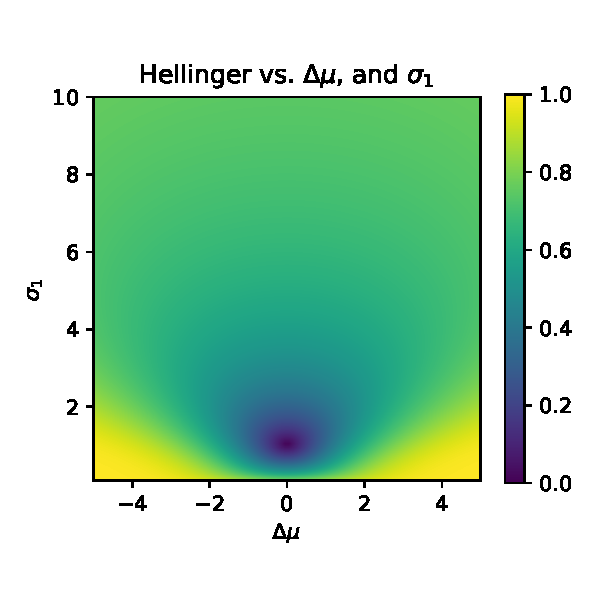
\includegraphics[width=0.9\linewidth]{Figures/hellinger_surf}
    \caption{Visualization of how the Hellinger distance varies with $\Delta\mu=\mu_1-\mu_2$ and $\sigma_1$ when $\mu_2=0.0$ and $\sigma_2=1.0$}
    \label{fig:hellinger_surf}
\end{figure}
\begin{figure}[tbp]
    \centering
    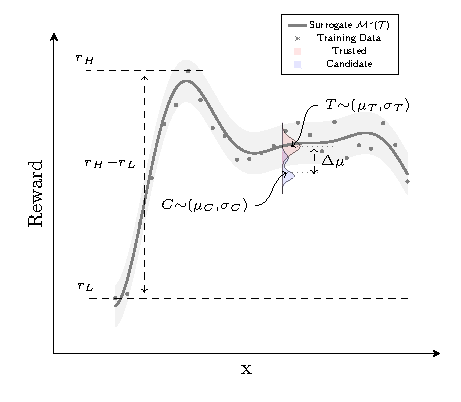
\includegraphics[width=0.9\linewidth]{build/sq_v2_fig}
    \caption{Figure that graphically depicts the key values involved in calculating SQ.}
    \label{fig:hellinger_surf}
\end{figure}

Using the Hellinger distance we are able to quantify how much the trusted and candidate distributions overlap. However, there are a couple of other considerations that need to be taken into account. First, is that since the Hellinger distance is a distance measure it is always greater than zero, and so information that indicates if a distribution is better or worse is lost. In order to address this we use the sign of the difference between the two distributions $(\mu_1-\mu_2)$.

The next consideration is that just because distance between two distributions may be great or small, does not mean that in the big picture the difference is actually that great. In the extreme case one might imagine two Normal distributions with means $\mu_1=1$ and $\mu_2=2$, and low variances $\sigma_1=\sigma_2=1e\-5$. In this case the Hellinger distance between the two would be 1 since they share practically no overlapping probability. However, if the means of the distributions are nearly equal on the global scale (for example if range of interest is between $[-1e3,1e3]$), then the quantity of the Hellinger distance isn't as important.

Incorporating all of these ideas together yields the equation for solver quality:

\begin{align}
    \Delta \mu &= \mu_c-\mu_t\\
    f &= \Delta \mu/(r_H-r_L) \label{eq:f}\\
    \text{sq} &= \text{sgn}(\Delta \mu)f^{\alpha}\sqrt{H_{\mathcal{N}}^{2}(P,Q)} \label{eq:sq}
\end{align}

The exponent $\alpha$ is a parameter that affects the influence that $f$ has with respect to $H_{\mathcal{N}}$. Basically, should the relationship between $f$ and $H_{\mathcal{N}}$ be $1\to1$? In practice $\alpha=1$ does not yield desirable results. Hellinger distance should be more influential on $\text{sq}$ as $f$ grows smaller, and $f$ should be more influential as it increases. The effects of different values of $\alpha$ are illustrated in Figure \ref{fig:alphas}. We have found $\alpha=1/2$ gives results that `make sense' to users; future work could investigate the `best' value for $\alpha$ via user studies.

\begin{figure}[tbp]
    \centering
    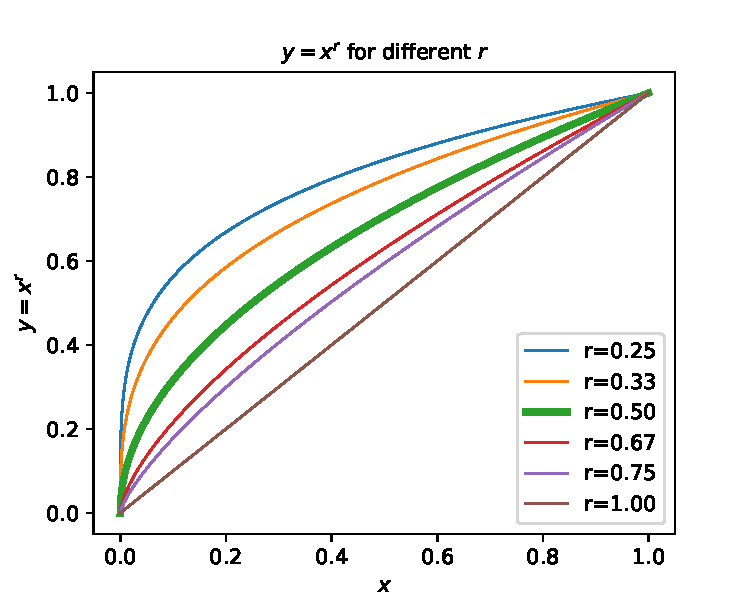
\includegraphics[width=0.9\linewidth]{Figures/power_comparison}
    \caption{Relative effects of different values of $\alpha$.}
    \label{fig:alphas}
\end{figure}

While the Hellinger distance is on the domain $[0,1]$, the quantity $f$ from Equation \ref{eq:f} is $[0,\infty]$. Because of this it is desirable to use a `squashing function' to keep SQ value within some range and avoid arbitrarily large values that can be confusing to users. The general logistic equation is useful for this:

\begin{align}
    y &= \frac{L}{1+exp(-k(x-x_0))} \label{eq:get_log}
\end{align}

We use $L=2$ so that when $s=0$ (distributions are identical) SQ will be 1. The parameter $k$ is selected to be $5$ so that SQ `saturates' at around $SQ=\pm1$ (see Figure \ref{fig:log_sat}).
\begin{align}
    \text{SQ} &= \frac{2}{1+exp(-\text{sq}/5)}\label{eq:SQ}
\end{align}
\begin{figure*}[tbp]
    \centering
    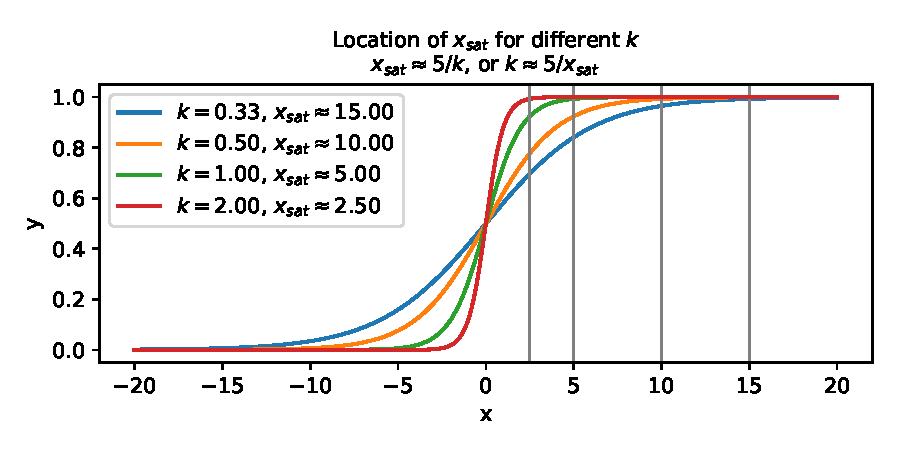
\includegraphics[width=0.9\linewidth]{Figures/logistic_saturation}
    \caption{Illustration of the behavior of the logistic function given different values of $k$. With $k=1$ the function reaches `saturation' at around $\pm5$. This `saturation' point $x_{sat}\approx 5/k$ helps to design SQ to be able have the right scale when comparing distributions.}
    \label{fig:log_sat}
\end{figure*}

Figure \ref{fig:sq_surf} shows the behavior of SQ when $\sigma_1=1.0,\mu_2=0.0,\sigma_2=1.0$, and $\mu_1$ and $f$ vary.

\begin{figure}[tbp]
    \centering
    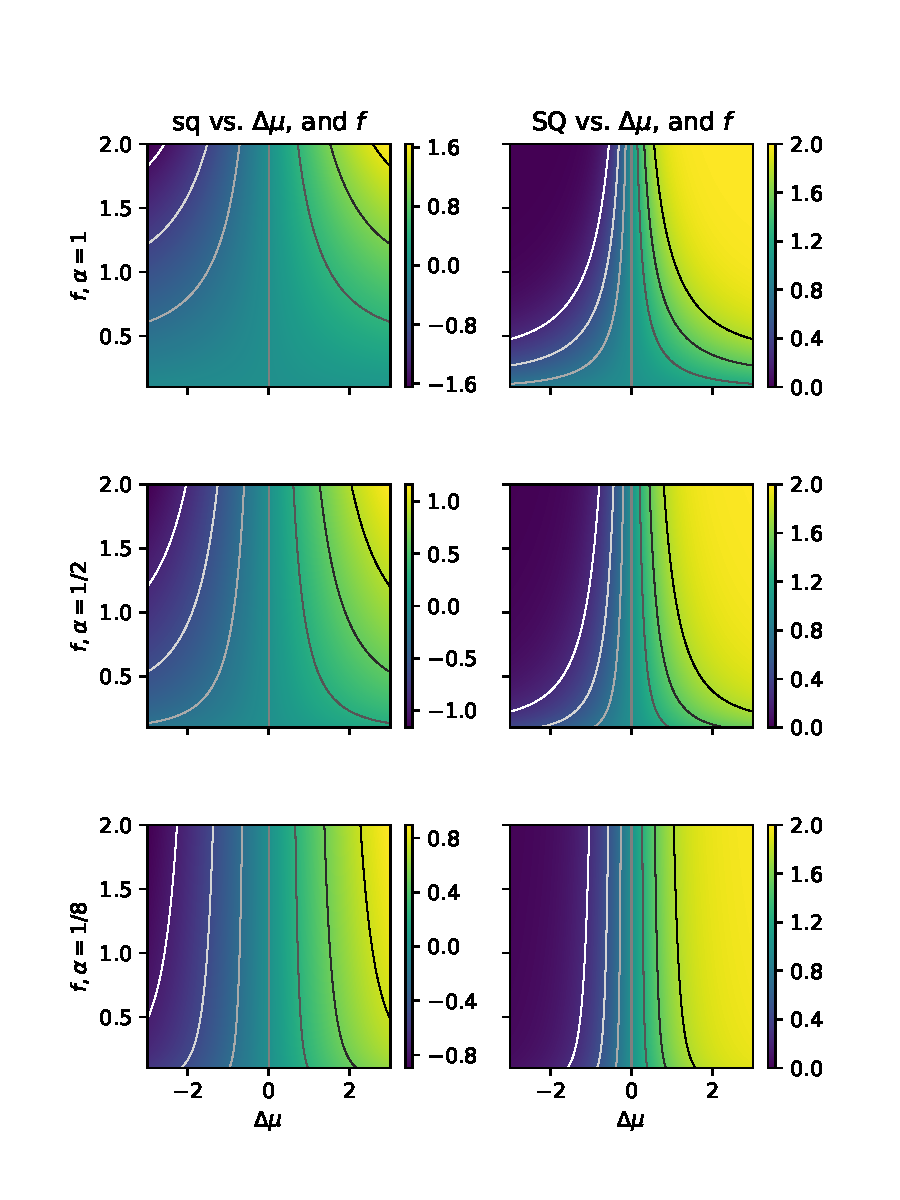
\includegraphics[width=0.9\linewidth]{Figures/sq_surf}
    \caption{Variation in SQ based on change in $\mu_1$ and $f$ compared for different values of $\alpha$.}
    \label{fig:sq_surf}
\end{figure}

\subsection{Examples}
It is easiest to show results of this calculation on some simple examples. Figure \ref{fig:sq_thry1} is a toy example showing the expected reward (with uncertainty) for a trusted solver given a specific task parameter, as well as that of a `candidate' solver. Different points of interest (indicating specific values of the task parameter) are highlighted by a star.

Figure \ref{fig:sq_thry2} shows a cross-section of the graph at the corresponding value of the task parameter. \textbf{talk a bit more here about each of the examples}.

\begin{figure}[tbp]
    \centering
    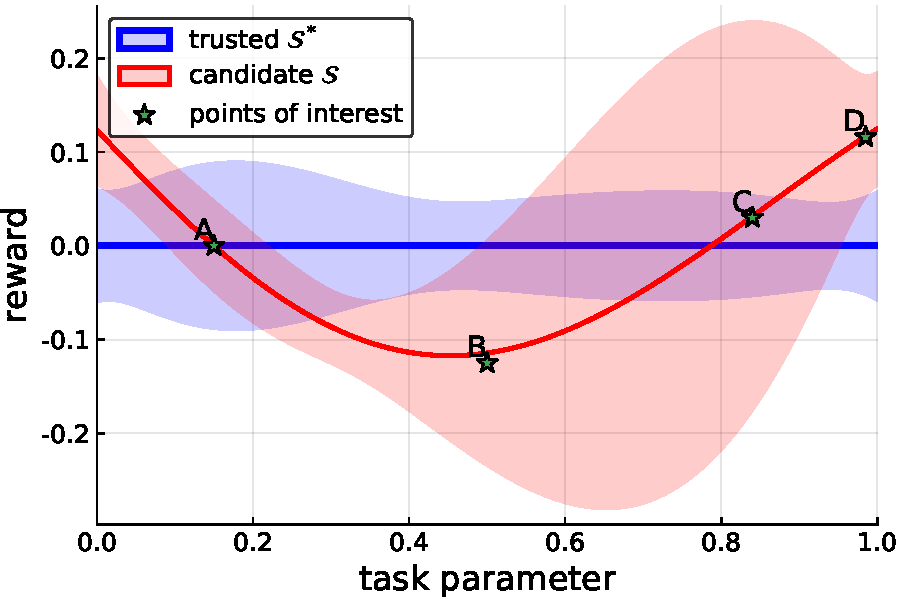
\includegraphics[width=0.9\linewidth]{Figures/p1}
    \caption{example of expected rewards of solvers versus variation of a problem parameter}
    \label{fig:sq_thry1}
\end{figure}

\begin{figure}[tbp]
    \centering
    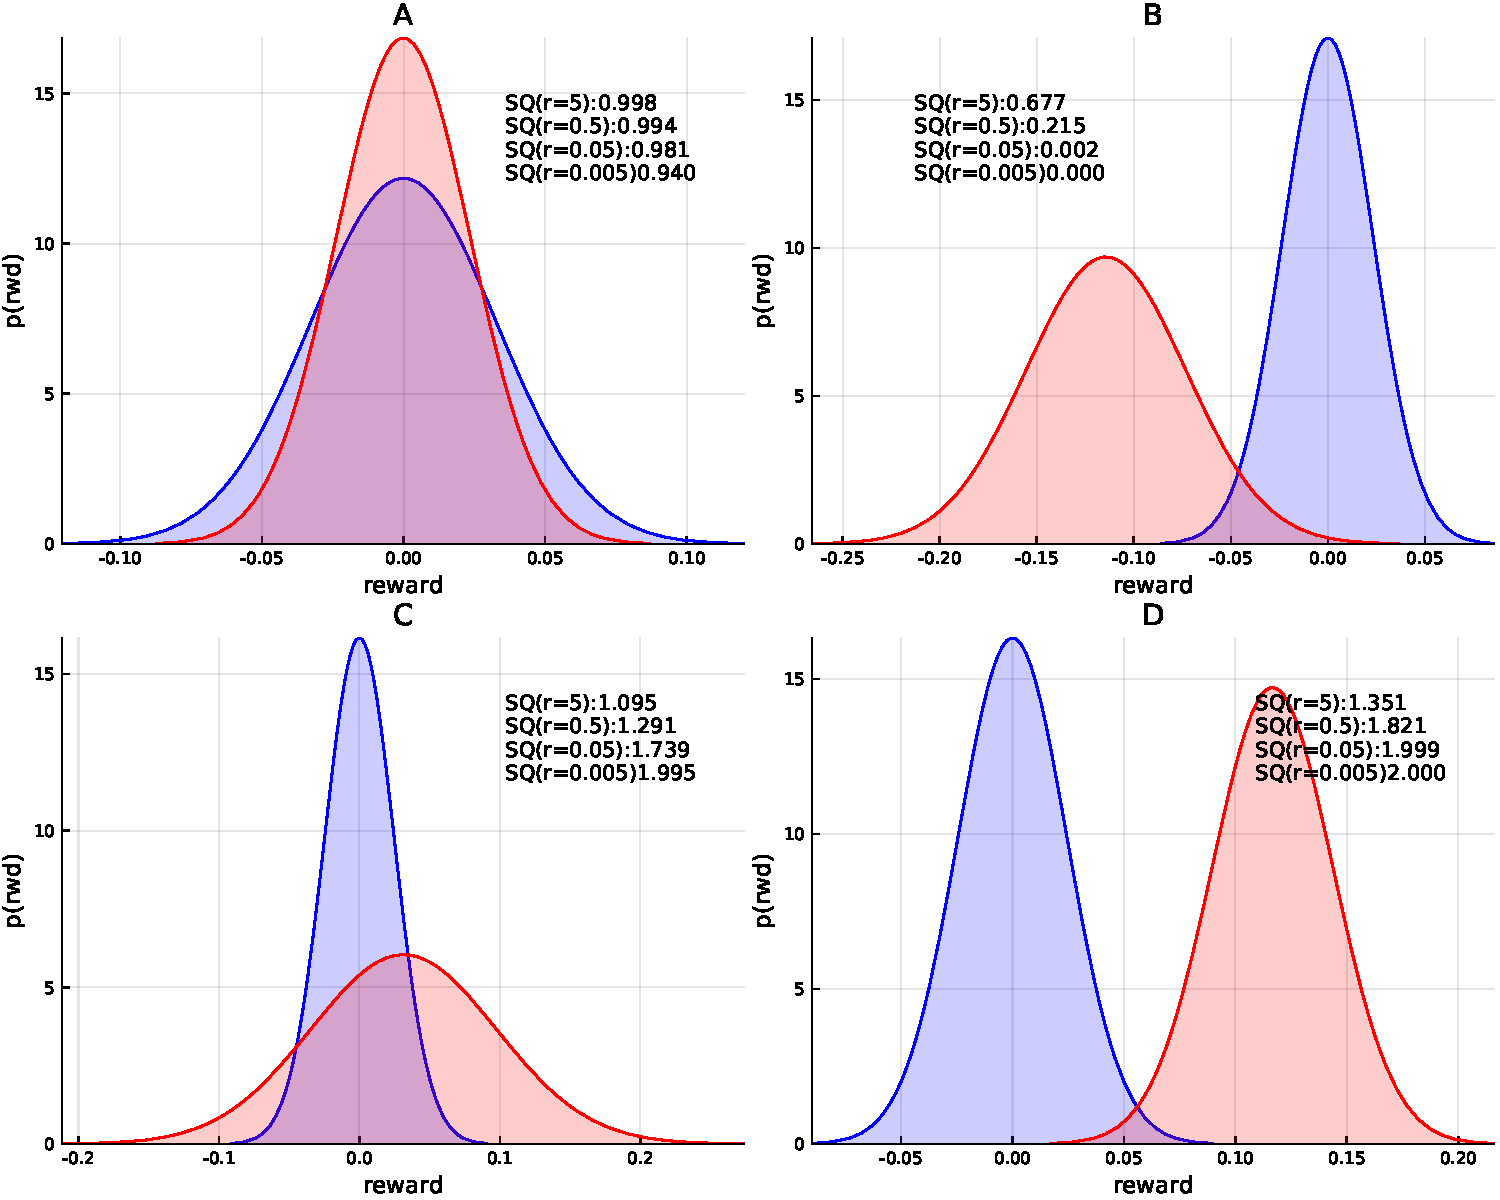
\includegraphics[width=0.9\linewidth]{Figures/point_compare}
    \caption{Plots depicting the distributions at each of the points indicated in \ref{fig:sq_thry1}. Solver quality (SQ) values are shown for several different values of the solver reward range $r$}
    \label{fig:sq_thry2}
\end{figure}
